\documentclass[10pt]{beamer}	
%\documentclass[10pt,aspectratio=43,mathserif]{beamer}		
%设置为 Beamer 文档类型,设置字体为 10pt,长宽比为16:9,数学字体为 serif 风格
%\documentclass[handout]{beamer}

\usepackage{seu}
\usepackage{amsmath,amsfonts,amssymb,bm}
\usepackage{color}
\usepackage{graphicx,hyperref,url}	
\usepackage[utf8]{inputenc}
\usepackage[main=english]{babel} 

\title[\textbf{Operating System Concepts}]{\textbf{OPERATING SYSTEM CONCEPTS}}
\subtitle{\textbf{Chapter 6. Process Synchronization}}
\author{\textbf{A/Prof.\ Kai Dong}}

\institute[CSE@SEU]{
{dk@seu.edu.cn}\\
  School of Computer Science and Engineering,\\Southeast University}

\date{\scriptsize \today}

\usepackage{tikz}
\usetikzlibrary{calc, shapes, backgrounds}

% used within this chapter
\usepackage{marvosym}
\usepackage{listings}
\usepackage{xcolor}
\definecolor{mygreen}{rgb}{0,0.6,0}
\definecolor{mygray}{rgb}{0.5,0.5,0.5}
\definecolor{mymauve}{rgb}{0.58,0,0.82}
\lstset{basicstyle=\tiny, breaklines=true, numbers=left, numberstyle=\tiny\color{mygray}, keywordstyle=\color{blue}, commentstyle=\color{mygreen}, frame=shadowbox, rulesepcolor=\color{black}, stringstyle=\color{mymauve}, escapeinside={(*@}{@*)}, xleftmargin=2em, xrightmargin=2em, aboveskip=0em}

\setbeamertemplate{itemize/enumerate body begin}{\footnotesize}
\setbeamertemplate{itemize/enumerate subbody begin}{\footnotesize}
\setbeamertemplate{itemize/enumerate subsubbody begin}{\footnotesize}

\begin{document}
\begin{frame}[label=title]
\titlepage\end{frame}

 \AtBeginSection[]{
 \begin{frame}<beamer>
 \frametitle{Contents}
 \tableofcontents[sectionstyle=show/shaded]
 \end{frame}}

\section[0.Prologue]{Warm-up}
\begin{frame}[fragile]{Warm-up}
\framesubtitle{What is the Output?}
\begin{minipage}{.49\linewidth}
\begin{lstlisting}[language=C]
/* thread.c */
#include <stdio.h>
#include <stdlib.h>
#include <common.h>

volatile int counter = 0;
int loops;

void *worker(void *arg) {
 int i;
 for (i = 0; i < loops; i++) {
 counter++;
 }
 return NULL;
}
\end{lstlisting}
\end{minipage}
\hspace{13pt}
\begin{minipage}{.49\linewidth}
\begin{lstlisting}[language=C]
int main(int argc, char *argv[]) {
 if (argc != 2) {
 fprintf(stderr, "usage: threads <value>\n");	
 exit(1);
 }
 loops = atoi(argv[1]);
 pthread_t p1, p2;
 printf("Initial value : %d\n", counter);

 Pthread_create(&p1, NULL, worker, NULL);
 Pthread_create(&p2, NULL, worker, NULL);
 Pthread_join(p1, NULL);
 Pthread_join(p2, NULL);
 printf("Final value : %d\n", counter);
 return 0;
}
\end{lstlisting}
\end{minipage}
\end{frame}

\begin{frame}[fragile]{Warm-up}
\framesubtitle{Concurrency}
\begin{lstlisting}[language=sh]
prompt> gcc -o thread thread.c -Wall -pthread
prompt> ./thread 1000
Initial value : 0
Final value : 2000

prompt> ./thread 100000
Initial value : 0
Final value : 143012
prompt> ./thread 100000
Initial value : 0
Final value : 137298
\end{lstlisting}
\begin{itemize}
\item \textbf{\alert{Concurrency}} --- Many problems arise, and must be addressed, when working on many things at once (i.e., concurrently) in the same program.
\end{itemize}
\end{frame}

\begin{frame}{Objectives}
\begin{itemize}
\item To present the concept of process synchronization.
\item To introduce the critical-section problem, whose solutions can be used to ensure the consistency of shared data
\item To present both software and hardware solutions of the critical-section problem
\item To examine several classical process-synchronization problems
\item To explore several tools that are used to solve process synchronization problems
\end{itemize}
\end{frame}



\section[1.Background]{Background}
\begin{frame}{Background}
\begin{itemize}
\item Processes (and threads) can execute concurrently
\begin{itemize}
\item May be interrupted at any time, partially completing execution
\end{itemize}
\item Concurrent access to shared data may result in data inconsistency
\item Maintaining data consistency requires mechanisms to ensure the orderly execution of cooperating processes
\item In our warm-up example, what data is shared?
\end{itemize}
\end{frame}

\begin{frame}[fragile]{Background}
\framesubtitle{Result Indeterminate}
\begin{itemize}
\item One line of C code
\begin{lstlisting}[language=C]
counter ++
\end{lstlisting}
\item is compiled as
\begin{uncoverenv}
\begin{lstlisting}[language={[x86masm]Assembler}] 
mov 0x8049a1c, %eax	; register1 = counter
add $0x1, %eax	    ; register1 = register1 + 1
mov %eax, 0x8049a1c	; counter = register1
\end{lstlisting}
\end{uncoverenv}
\item Consider this execution interleaving with $counter = 50$ initially:
\begin{uncoverenv}
\begin{table}
\scriptsize
\begin{tabular}{l l l}
$S0:$&p1 executes register1 = counter&(register1 = 50)\\
$S1:$&p1 executes register1 = register1 + 1&(register1 =51)\\
$S2:$&p2 executes register2 = counter&(register2 = 50)\\
$S3:$&p2 executes register2 = register2 + 1&(register2 = 51)\\
$S4:$&p1 executes counter = register1&(counter = 51)\\
$S5:$&p2 executes counter = register2&(counter = 51 \textcolor{blue}{NOT 52})\\
\end{tabular}
\end{table}
\end{uncoverenv}
\item Because of multi-processors? Not really.
\end{itemize}
\end{frame}

\begin{frame}{Background}
\framesubtitle{Uncontrolled Scheduling}
\centering
\scriptsize
\begin{tabular}{l l l c c c}
&&&\multicolumn{3}{c}{(after instruction)}\\
\textbf{OS}&\textbf{Thread 1}&\textbf{Thread 2}&\textbf{PC}&\textbf{\%eax}&\textbf{counter}\\
\hline
&\emph{before critical section}&&100&0&50\\
&mov 0x8049a1c, \%eax&&105&50&50\\
&add \$0x1, \%eax&&108&51&50\\
\textbf{interrupt}&&&&&\\
\quad\emph{save T1's state}&&&&&\\
\quad\emph{restore T2's state}&&&100&0&50\\
&&mov 0x8049a1c, \%eax&105&50&50\\
&&add \$0x1, \%eax&108&51&50\\
&&mov \%eax, 0x8049a1c&113&51&51\\
\textbf{interrupt}&&&&&\\
\quad\emph{save T2's state}&&&&&\\
\quad\emph{restore T1's state}&&&108&51&50\\
&mov \%eax, 0x8049a1c&&113&51&51\\
\end{tabular}
\begin{itemize}
 
\item The heart of the problem: uncontrolled scheduling
\item What if we had a super instruction \textcolor{blue}{``memory-add 0x8049a1c, \$0x1''}?
\end{itemize}
\end{frame}

\begin{frame}{Background}
\framesubtitle{Race Condition}
\begin{itemize}
\item \textbf{\alert{Race condition}}
\begin{itemize}
\item Several processes (threads) access and manipulate the same data concurrently and the outcome of the execution depends on the particular order in which the access takes place.
\item \alert{Result indeterminate}
\end{itemize}
\end{itemize}
\end{frame}

\section[2.CS Prob.]{The Critical-Section Problem}
\begin{frame}{The Critical-Section Problem}
\begin{itemize}
 
\item Consider system of $n$ processes $P_0, P_1, \cdots, P_{n-1}$
\item Each process has \textbf{\alert{critical section}} segment of code
\begin{itemize}
\item Process may be changing common variables, updating table, writing file, etc
\item When one process in critical section, no other may be in its critical section
\end{itemize}
\item \textbf{\alert{Critical section}}
\begin{itemize}
\item Multiple threads executing a segment of code, which can result in a \textbf{\alert{race condition}}.
\item Question: what codes are in critical section in previous examples?
\end{itemize}
\item \textbf{\alert{Critical section problem}} is to design protocol to avoid race condition.
\item Each process must ask permission to enter critical section in \textbf{\alert{entry section}}, may follow critical section with \textbf{\alert{exit section}}, then \textbf{\alert{remainder section}}
\end{itemize}
\end{frame}

\begin{frame}[fragile]{The Critical-Section Problem}
\begin{itemize}
\item General structure of process $P_i$
\vspace{6pt}\\
\begin{lstlisting}[language=C]
do {
	[entry section]
		[critical section]
	[exit section]
		[remainder section]
} while (true);
\end{lstlisting}
\item An algorithm for process $P_i$ and $P_j$
\vspace{6pt}\\
\begin{minipage}{.49\linewidth}
\begin{lstlisting}[language=C]
do {
    while (turn == j); 
        critical section 
    turn = j; 
        remainder section 
} while (true);
\end{lstlisting}
\end{minipage}
\hspace{13pt}
\begin{minipage}{.49\linewidth}
\begin{lstlisting}[language=C]
do {
    while (turn == i); 
        critical section 
    turn = i; 
        remainder section 
} while (true);
\end{lstlisting}
\end{minipage}
\item \textcolor{blue}{Is it a correct solution?}
\end{itemize}
\end{frame}

\begin{frame}{The Critical-Section Problem}
\framesubtitle{Solution to Critical-Section Problem}
\begin{enumerate}
 
\item \textbf{\alert{Mutual Exclusion}} --- If process $P_i$ is executing in its critical section, then no other processes can be executing in their critical sections
\item \textbf{\alert{Progress}} --- If no process is executing in its critical section and there exist some processes that wish to enter their critical section, then the selection of the processes that will enter the critical section next cannot be postponed indefinitely
\item \textbf{\alert{Bounded Waiting}} --- A bound must exist on the number of times that other processes are allowed to enter their critical sections after a process has made a request to enter its critical section and before that request is granted
\begin{itemize}
\item Assume that each process executes at a nonzero speed 
\item No assumption concerning relative speed of the $n$ processes
\end{itemize}
\end{enumerate}
\end{frame}

\begin{frame}{The Critical-Section Problem}
\framesubtitle{Critical Section Handling in OS}
\begin{itemize}
 
\item Two approaches depending on if kernel is preemptive or non-preemptive
\begin{itemize}
\item \textcolor{blue}{Preemptive} --- allows preemption of process when running in kernel mode
\item \textcolor{blue}{Non-preemptive} --- runs until exits kernel mode, blocks, or voluntarily yields CPU
\begin{itemize}
\item Essentially free of race conditions in kernel mode
\end{itemize}
\end{itemize}
\item Why would anyone favor a preemptive kernel over a non-preemptive one?
\begin{itemize}
\item A preemptive kernel may be more responsive, since there is less risk that a kernel-mode process will run for an arbitrarily long period before relinquishing the processor to waiting processes. 
\end{itemize}
\end{itemize}
\end{frame}

\section[3.Mutex]{Mutex Locks}
\begin{frame}{Mutex Locks}
\framesubtitle{Controlling Scheduling}
\begin{itemize}
 
\item What we need: \alert{Hardware synchronization primitives}.
\begin{itemize}
\item \textbf{\alert{Lock}}-related source codes are put around critical sections, thus ensure that any such critical section executes as if it were a single \textcolor{blue}{atomic} instruction.
\end{itemize}
\item A lock is just a \textcolor{blue}{variable}.
\item How to use a lock:
\begin{itemize}
\item Declare a \textcolor{blue}{lock variable} (e.g., $mutex$).
\item The lock variable holds \textcolor{blue}{the state of the lock}.
\item It is either available (or \textcolor{blue}{unlocked} or free), means that no thread holds the lock;
\item Or acquired (or \textcolor{blue}{locked} or held), means that exactly one thread holds the lock.
\end{itemize}
\end{itemize}
\end{frame}

\begin{frame}[fragile]{Mutex Locks}
\framesubtitle{Locks}
\begin{itemize}
\item Algorithm for process $P_i$
\vspace{6pt}\\
\begin{lstlisting}[language=C]
do { 
	lock();
		critical section 
	unlock(); 
		remainder section 
} while (true); 
\end{lstlisting}
\item The semantic of the $lock$() and $unlock$() routines?
\end{itemize}
\end{frame}

\begin{frame}{Mutex Locks}
\framesubtitle{Semantic of $lock$() and $unlock$() Routines}
\begin{itemize}
 
\item The semantic of the \textcolor{blue}{$lock$()} routines.
\begin{itemize}
 
\item Calling the routine $lock$() tries to acquire the lock.
\item If no other thread holds the lock (i.e., it is free), the thread will acquire the lock and enter the critical section; this thread is sometimes said to be the owner of the lock.
\item If another thread then calls $lock$() on that same lock variable, it will not return since the lock is held by its owner.
\item Other threads are prevented from entering the critical section while the first thread that holds the lock is in there.
\end{itemize}
\item The semantic of the \textcolor{blue}{$unlock$()} routines.
\begin{itemize}
 
\item Once the owner of the lock calls $unlock$(), the lock is now available (free) again.
\item If no other threads are waiting for the lock, the state of the lock is simply changed to free; otherwise, one of the waiting threads will notice this change of the lock's state, acquire the lock, and enter the critical section.
\end{itemize}
\end{itemize}
\end{frame}

\begin{frame}[fragile]{Mutex Locks}
\framesubtitle{Pthread Locks}
\begin{itemize}
 
\item Entry \& Exit
\vspace{6pt}\\
\begin{lstlisting}[language=C]
int pthread_mutex_lock(pthread_mutex *mutex);
int pthread_mutex_unlock(pthread_mutex *mutex);
\end{lstlisting}
\item initialization
\vspace{6pt}\\
\begin{uncoverenv}
\begin{lstlisting}[language=C]
pthread_mutex_t lock = PTHREAD_MUTEX_INITIALIZER;
int rc = pthread_mutex_init(&lock, NULL);
assert(rc == 0);
\end{lstlisting}
\end{uncoverenv}
\item Destruction
\vspace{6pt}\\
\begin{uncoverenv}
\begin{lstlisting}[language=C]
pthread_mutex_destroy(&lock);
pthread_mutex_destroy(lock);
\end{lstlisting}
\end{uncoverenv}
\item Other versions
\vspace{6pt}\\
\begin{uncoverenv}
\begin{lstlisting}[language=C]
int pthread_mutex_trylock(pthread_mutex_t *mutex);
int pthread_mutex_trylock(pthread_mutex_t *mutex, struct timespec *abs_timeout);
\end{lstlisting}
\end{uncoverenv}
\end{itemize}
\end{frame}

\begin{frame}{Mutex Locks}
\framesubtitle{Building A Lock}
\begin{itemize}
 
\item How can OS build an efficient lock? 
\begin{itemize}
\item It depends, on which hardware synchronization primitives are used.
\end{itemize}
\item Ways of Building A Lock
\begin{itemize}
\item Without special hardware support
\begin{itemize}
\item \textcolor{red}{Dekker's and Peterson's Algorithms}
\item Lamport's Bakery Algorithm
\end{itemize}
\item With hardware support
\begin{itemize}
\item Controlling Interrupts
\item \textcolor{red}{The test-and-set instruction} (atomic exchange)
\item The compare-and-swap instruction (compare-and-exchange)
\item \textcolor[rgb]{.5,.5,.5}{Load-Linked and Store-Conditional}
\item \textcolor[rgb]{.5,.5,.5}{Fetch-And-Add}
\end{itemize}
\end{itemize}
\item Discussion on \textcolor{red}{spin-waiting}  
\end{itemize}
\end{frame}

\begin{frame}[fragile]{Mutex Locks}
\framesubtitle{Controlling Interrupts}
\begin{itemize}
\item For single-processor systems:
\begin{itemize}
\item One of the earliest solutions used to provide mutual exclusion was to disable interrupts for critical sections.
\vspace{6pt}\\
\begin{uncoverenv}
\begin{lstlisting}[language=C]
void lock() {
	DisableInterrupts();
}
void unlock() {
	EnableInterrupts();
}
\end{lstlisting}
\end{uncoverenv}
\item $Disable/EnableInterrupts$() are implemented by using special hardware instructions.
\end{itemize}
\item \textcolor{blue}{Question: Is it a solution to the critical section problem?}
\begin{itemize}
\item Whether or not it satisfies: Mutual exclusion? Progress? Bounded Waiting?
\end{itemize}
\item And what about Performance?
\end{itemize}
\end{frame}

\begin{frame}{Mutex Locks}
\framesubtitle{Controlling Interrupts (contd.)}
\begin{itemize}
 
\item What are the \textbf{\textcolor{blue}{negatives}}?
\item This approach requires us to allow any calling thread to perform a \textcolor{blue}{privileged operation} (turning interrupts on/off), and trust this facility is not abused.
\begin{itemize}
 
\item A greedy program could call lock() at the beginning of its execution and thus monopolize the processor; worse, an errant or malicious program could call lock() and go into an endless loop.
\end{itemize}
\item This approach does \textcolor{blue}{not work on multiprocessors}.
\begin{itemize}
 
\item Threads will be able to run on other processors, and thus could enter the critical section.
\end{itemize}
\item This approach may \textcolor{blue}{lost interrupts}.
\begin{itemize}
 
\item E.g., if the CPU missed the fact that a disk device has finished a read request. How will the OS know to wake the process waiting for said read?
\end{itemize}
\item This approach can be \textcolor{blue}{inefficient}.
\begin{itemize}
 
\item Codes that mask or unmask interrupts are executed slowly.
\end{itemize}
\end{itemize}
\end{frame}

\begin{frame}[fragile]{Mutex Locks}
\framesubtitle{Peterson's Solution}
\begin{itemize}
 
\item Good algorithmic description of solving the problem
\item Two process solution
\item \textcolor{blue}{Assume that the \alert{load} and \alert{store} machine-language instructions are atomic; that is, cannot be interrupted.}
\item The two processes share two variables:
\vspace{6pt}\\
\begin{uncoverenv}
\begin{lstlisting}[language=C]
int turn;
Boolean flag[2];
\end{lstlisting}
\end{uncoverenv}
\item The variable $turn$ indicates whose turn it is to enter the critical section
\item The $flag$ array is used to indicate if a process is ready to enter the critical section. $flag[i] = true$ implies that process $P_i$ is ready!
\end{itemize}
\end{frame}

\begin{frame}[fragile]{Mutex Locks}
\framesubtitle{Peterson's Solution (contd.)}
\centering
\begin{minipage}{.45\linewidth}
\centering
Algorithm for Process $P_i$
\end{minipage}
\hspace{13pt}
\begin{minipage}{.45\linewidth}
\centering
Algorithm for Process $P_j$
\end{minipage}
\vspace{6pt}\\
\begin{minipage}{.49\linewidth}
\begin{lstlisting}[language=C]
do {
 flag[i] = true;
 turn = j;
 while (flag[j] && turn == j);
 critical section
 flag[i] = false;
 remainder section
} while (true);
\end{lstlisting}
\end{minipage}
\hspace{13pt}
\begin{minipage}{.49\linewidth}
\begin{lstlisting}[language=C]
do {
 flag[j] = true;
 turn = i;
 while (flag[i] && turn == i);
 critical section
 flag[j] = false;
 remainder section
} while (true);
\end{lstlisting}
\end{minipage}
\begin{itemize}
\item \textcolor{blue}{Prove that the algorithm satisfies all requirements for the critical section problem}
\end{itemize}
\end{frame}

\begin{frame}[fragile]{Mutex Locks}
\framesubtitle{Why Failed?}
\begin{itemize}
 
\item Failed attempt $\sharp 1$
\vspace{2pt}\\
\begin{lstlisting}[language=C]
do {	while (flag[j]);
	flag[i] = true;
		critical section
	flag[i] = false;
		remainder section	} while (true);
\end{lstlisting}
\item Failed attempt $\sharp 2$
\vspace{2pt}\\
\begin{uncoverenv}
\begin{lstlisting}[language=C]
do {	flag[i] = true;
	while (flag[j]);
		critical section
	flag[i] = false;
		remainder section	} while (true);
\end{lstlisting}
\end{uncoverenv}
\item Failed attempt $\sharp 3$
\vspace{2pt}\\
\begin{uncoverenv}
\begin{lstlisting}[language=C]
do {	victim = i;
	while (victim == i);
		critical section
		remainder section	} while (true);
\end{lstlisting}
\end{uncoverenv}
\end{itemize}
\end{frame}

\begin{frame}{Mutex Locks}
\framesubtitle{Why Failed? (Failed attemp $\sharp 1$)}
\scriptsize
\begin{tabular}{|l|c|}
\hline
Mutual exclusion & F\\
Progress & T\\
Bounded waiting & F\\
\hline
\end{tabular}
\\
\vspace{2em}
\centering
\begin{tabular}{l l}
\textbf{Thread 1}&\textbf{Thread 2}\\
\hline
while(flag[2]); &\\
\textbf{interrupted: switch to Thread 2}&\\
& while(flag[1]); \\
& flag[2] = true; \\
& critical section \\
& \textbf{interrupted: switch to Thread 1}\\
flag[1] = true; &\\
critical section &\\
\end{tabular}
\end{frame}

\begin{frame}{Mutex Locks}
\framesubtitle{Why Failed? (Failed attemp $\sharp 2$)}
\scriptsize
\begin{tabular}{|l|c|}
\hline
Mutual exclusion & T\\
Progress & F\\
Bounded waiting & T\\
\hline
\end{tabular}
\\
\vspace{2em}
\centering
\begin{tabular}{l l}
\textbf{Thread 1}&\textbf{Thread 2}\\
\hline
&flag[2] = true;\\
& \textbf{interrupted: switch to Thread 1}\\
flag[1] = true;&\\
while (flag[2]) &\\
\textbf{blocked: switch to Thread 2} &\\
& while (flag[1])\\
& \textbf{blocked: switch to Thread 1}\\
$\cdots$ &\\
\end{tabular}
\end{frame}

\begin{frame}{Mutex Locks}
\framesubtitle{Why Failed? (Failed attemp $\sharp 3$)}
\scriptsize
\begin{tabular}{|l|c|}
\hline
Mutual exclusion & T\\
Progress & F\\
Bounded waiting & T\\
\hline
\end{tabular}
\\
\vspace{2em}
\centering
\begin{tabular}{l l}
\textbf{Thread 1}&\textbf{Thread 2}\\
\hline
remainder section&\\
(performing I/O) &\\
\textbf{blocked: switch to Thread 2}&\\
&victim = 2;\\
&while (victim == 2) \\
&\textbf{blocked: switch to Thread 1}\\
$\cdots$ &\\
(I/O interrupt) &\\
victim = 1;&\\
$\cdots$ &\\
\end{tabular}
\end{frame}


\begin{frame}{Mutex Locks}
\framesubtitle{Bakery Algorithm}
\begin{itemize}
 
\item Peterson's solution is restricted to two processes that alternate execution between their critical sections and remainder sections. 
\item What if there are more than two cooperating processes?
\item Bakery Algorithm --- Critical section for $n$ processes
\item Lamport envisioned a bakery with a numbering machine at its entrance so each \textcolor{blue}{customer} is given a \textcolor{blue}{unique number}. Numbers increase by one as customers enter the store. A \textcolor{blue}{global counter} displays the number of the customer that is currently being served. All other customers must \textcolor{blue}{wait in a queue} until the baker finishes serving the current customer and the next number is displayed. When the customer is done shopping and has disposed of his or her number, the clerk increments the number, allowing the next customer to be served. That customer must draw another number from the numbering machine in order to shop again.
\end{itemize}
\end{frame}

\begin{frame}[fragile]{Mutex Locks}
\framesubtitle{Bakery Algorithm}
\begin{itemize}
 
\item Before entering its critical section, process (\textcolor{blue}{customer}) receives a number. Holder of the smallest number enters the critical section. (\textcolor{blue}{wait in a queue})
\item If processes $P_i$ and $P_j$ receive the same number, if $i < j$, then $P_i$ is served first; else $P_j$ is served first. (\textcolor{blue}{a unique number})
\item The numbering scheme always generates numbers in increasing order of enumeration; e.g., $1,2,3,3,3,3,4,5,\cdots$
\item Define two operators: 
\begin{itemize}
\item $(a,b) < (c,d)$ if $a < c$ or if $a = c$ and $b < d$
\item $\max (a_0,\cdots, a_{n-1})=k$, i.e., $k \geq a_i, \forall i\in[0,n]$
\end{itemize}
\item Shared data
\vspace{2pt}\\
\begin{uncoverenv}
\begin{lstlisting}[language=C]
boolean choosing[n];	// initialized to false
int number[n]; 	// initialized to 0
\end{lstlisting}
\end{uncoverenv}
\end{itemize}
\end{frame}

\begin{frame}[fragile]{Mutex Locks}
\framesubtitle{Bakery Algorithm (contd.)}
\begin{lstlisting}[language=C]
do { 
	choosing[i] = true;
	number[i] = max(number[0], number[1], (*@$\cdots$@*), number [n - 1]) + 1;
	choosing[i] = false;
	for (j = 0; j < n; j ++) {
		while (choosing[j]); 
		while ((number[j] != 0) && ((number[j], j) < (number[i], i))); 
	}
		critical section
	number[i] = 0;
		remainder section
} while (true);
\end{lstlisting}
\begin{itemize}
 
\item What part are entry section and exit section?
\item What codes are in $lock$() and $unlock$()?
\item What is the use of $choosing$[]? (why fail without $choosing[]$?)
\end{itemize}
\end{frame}

\begin{frame}{Mutex Locks}
\framesubtitle{Bakery Algorithm (Why fail without $choosing[]$?)}
\scriptsize
\begin{tabular}{|l|c|}
\hline
Mutual exclusion & F\\
Progress & T\\
Bounded waiting & T\\
\hline
\end{tabular}
\\
\vspace{2em}
\centering
\begin{tabular}{l l}
\textbf{Thread i}&\textbf{Thread j}\\
\hline
max($\cdots$) &\\
\textbf{interrupted: switch to Thread j} &\\
&number[j] = max($\cdots$)\\
&while ((\textcolor{blue}{number[i]!=0}) \&\& ($\cdots$))\\
&critical section\\
&\textbf{interrupted: switch to Thread i}\\
number[i] = max($\cdots$) & \\
while (($\cdots$) \&\& (\textcolor{blue}{(number[j],j)<(number[i],i)}))&\\
critical section&
\end{tabular}
\end{frame}

\begin{frame}{Mutex Locks}
\framesubtitle{Conclusion}
\begin{itemize}
 
\item Developing locks that work without special hardware support became all the rage for a while, giving theory-types a lot of problems to work on. 
\item This line of work became quite \textcolor{blue}{useless} when people realized it is much easier to assume a little hardware support.
\item Further, algorithms like the ones above don't work on modern hardware (due to \textcolor{blue}{relaxed memory consistency models}), thus making them even less useful than they were before.
\end{itemize}
\end{frame}

\begin{frame}[fragile]{Mutex Locks}
\framesubtitle{Motivation of Test-And-Set: Why Failed?}
\begin{itemize}
 
\item A failed attempt --- why failed?
\vspace{6pt}\\
\begin{lstlisting}[language=C]
typedef struct __lock_t { int flags; } lock_t;

void init(lock_t *mutex) {
	mutex->flag = 0;	// 0 -> lock is available, 1 -> held
}

void lock(lock_t *mutex) {
	while (mutex>flag == 1)	//TEST the flag
		;		// spin-wait (do nothing)
	mutex->flag = 1;	// now SET it!
}

void unlock(lock_t *mutex) {
	mutex->flag = 0;
}
\end{lstlisting}
\end{itemize}
\end{frame}

\begin{frame}{Mutex Locks}
\framesubtitle{Why Failed? (contd.)}
\scriptsize
\begin{tabular}{|l|c|}
\hline
Mutual exclusion & F\\
Progress & T\\
Bounded waiting & F\\
\hline
\end{tabular}
\\
\vspace{2em}
\centering
\begin{tabular}{l l}
\textbf{Thread 1}&\textbf{Thread 2}\\
\hline
call $lock$()&\\
while (flag == 1)&\\
\textbf{interrupt: switch to Thread 2}&\\
&call $lock$()\\
&while (flag == 1)\\
&flag = 1\\
& critical section\\
&\textbf{interrupt: switch to Thread 1}\\
flag = 1&\\
critical section&
\end{tabular}
\end{frame}

\begin{frame}[fragile]{Mutex Locks}
\framesubtitle{Test And Set}
\begin{itemize}
 
\item Hardware support: Some form of \textbf{\alert{test-and-set}} instruction.
\vspace{6pt}\\
\begin{lstlisting}[language=C]
int TestAndSet(int *old_ptr, int new) {
	int old = *old_ptr;
	*old_ptr = new;
	return old;
}
\end{lstlisting}
\item It returns the old value pointed to by the $ptr$, and simultaneously updates said value to $new$.
\item The key is that this sequence of operations is performed \alert{atomically}.
\item Test-and-set enables you to $test$ the old value (which is what is returned) while simultaneously $setting$ the memory location to a new value.
\item \textcolor{blue}{Question: Can you build a lock based on this instruction?}
\end{itemize}
\end{frame}

\begin{frame}[fragile]{Mutex Locks}
\framesubtitle{Test And Set (contd.)}
\begin{lstlisting}[language=C]
typedef struct __lock_t { int flag; } lock_t;

void init(lock_t *lock) {
	lock->flag = 0;	// 0 -> available, 1 -> held
}

void lock(lock_t *lock) {
	while (TestAndSet(&lock->flag, 1) == 1)
		;	// spin-waiting
}

void unlock(lock_t *lock) {
	lock->flag = 0;
}
\end{lstlisting}
\begin{itemize}
 
\item Evaluating this spin lock:
\begin{itemize}
\item Mutual exclusion?
\begin{uncoverenv}
\textcolor{blue}{Yes}
\end{uncoverenv}
\item Progress?
\begin{uncoverenv}
\textcolor{blue}{Yes}
\end{uncoverenv}
\item Bounded waiting?
\begin{uncoverenv}
\textcolor{blue}{No}
\end{uncoverenv}
\end{itemize}
\end{itemize}
\end{frame}

\begin{frame}[fragile]{Mutex Locks}
\framesubtitle{Compare And Swap}
\begin{itemize}
 
\item Hardware support: \textbf{\alert{compare-and-swap}} atomic instruction
\item To test whether the value at the address specified by $ptr$ is equal to $expected$; if so, update the memory location pointed to by $ptr$ with the $new$ value. If not, do nothing.
\vspace{6pt}\\
\begin{uncoverenv}
\begin{lstlisting}[language=C]
int CompareAndSwap(int *ptr, int expected, int new) {
	int actual = *ptr;
	if (actual == expected)
		*ptr = new;
	return actual;
}
\end{lstlisting}
\end{uncoverenv}
\item \textcolor{blue}{Question: Can you build a lock based on this instruction?}
\end{itemize}
\end{frame}

\begin{frame}[fragile]{Mutex Locks}
\framesubtitle{Compare And Swap (contd.)}
\begin{lstlisting}[language=C]
void lock(lock_t *lock) {
	while (CompareAndSwap(&lock->flag, 0, 1) == 1)
		;	// spin-waiting
}
\end{lstlisting}
\begin{itemize}
 
\item Evaluating this spin lock.
\begin{itemize}
\item Mutual exclusion?
\begin{uncoverenv}
\textcolor{blue}{Yes}
\end{uncoverenv}
\item Progress?
\begin{uncoverenv}
\textcolor{blue}{Yes}
\end{uncoverenv}
\item Bounded waiting?
\begin{uncoverenv}
\textcolor{blue}{No}
\end{uncoverenv}
\end{itemize}
\item Compare-and-swap is more powerful than test-and-set. Can be used to achieve lock-free synchronization.
\end{itemize}
\end{frame}

\begin{frame}[fragile]{Mutex Locks}
\framesubtitle{Compare And Swap (contd.)}
 
\begin{itemize}
\item Lock-free synchronization 
\item How to implement a concurrent counter?
\begin{itemize}
\item lock(); update counter; unlock();
\end{itemize}
\item \alert{Discussion: Can you build a Class like \emph{AtomicInteger}?}
\end{itemize}
\begin{lstlisting}[language=C]
int CompareAndSwap(int *ptr, int expected, int new) {
	int actual = *ptr;
	if (actual == expected) {
	 *ptr = new;
	 return 1;
	}
	return 0;
}
\end{lstlisting}
\end{frame}

\begin{frame}[fragile]{Mutex Locks}
\framesubtitle{Compare And Swap (contd.)}
 
\begin{itemize}
\item An alternative approach that does not require explicit locking:
\vspace{6pt}\\
\begin{lstlisting}[language=C]
void AtomicIncrement(int *counter, int amount) {
	do {
		int old = *counter;
	} while (CompareAndSwap(counter, old, old+amount) == 0);
}
\end{lstlisting}
\item Benefits: No deadlock can arise.
\item We will detail deadlocks later in Chapter 7.
\end{itemize}
\end{frame}

\begin{frame}[fragile]{Mutex Locks}
\framesubtitle{Load-Linked and Store-Conditional}
\begin{lstlisting}[language=C]
int LoadLinked(int *ptr) {
	return *ptr;
}

int StoreConditional(int *ptr, int value) {
	if (no one has updated *ptr since the LoadLinked to this address) {
		*ptr = value;
		return 1;	// success!
	} else return 0;	// failed to update
}

void lock(lock_t *lock) {
	while (true) {
		while (LoadLinked(&lock->flag) == 1)
			;	// spin-waiting
		if (StoreConditional(&lock->flag, 1) == 1)
			return;
	}
}

/* or a simplified version */
void lock(lock_t *lock) {
	while (LoadLinked(&lock->flag) || !StoreConditional(&lock->flag, 1))
		;		// spin-waiting
}
\end{lstlisting}
\end{frame}

\begin{frame}[fragile]{Mutex Locks}
\framesubtitle{How to Satisfy Bounded Waiting?}
\begin{lstlisting}[language=C]
/* C-like pseudo code */
Initially Boolean waiting[i] = false; lock = false;

lock() {
	waiting[i] = true;
	while (waiting[i] && (TestAndSet(lock, 1) == 1));
	waiting[i] = false;
}

unlock() {
	j = (i + 1) % n;
	while ((j != i) && !waiting[j])
		j = (j + 1) % n;
	if (j == i)
		lock = false;
	else
		waiting[j] = false;
}
\end{lstlisting}
\end{frame}

\begin{frame}[fragile]{Mutex Locks}
\framesubtitle{Fetch And Add}
\begin{itemize}
\item Atomically increments a value while returning the old value at a particular address. 
\end{itemize}
\begin{lstlisting}[language=C]
int FetchAndAdd(int *ptr) {
	int old = *ptr;
	*ptr = old + 1;
	return old;
}

/* ticket lock */
typedef struct __lock_t { int ticket; int turn; } lock_t;
void lock_init(lock_t *lock) {
	lock->ticket = 0;
	lock->turn = 0;
}
void lock(lock_t *lock) {
	int myturn = FetchAndAdd(&lock->ticket);
	while (lock->turn != myturn);
}
void unlock(lock_t *lock) {
	lock->turn = lock->turn + 1;
}
\end{lstlisting}
\end{frame}

\begin{frame}{Mutex Locks}
\framesubtitle{Spin-Waiting}
\begin{itemize}
 
\item When a thread waits to acquire a lock that is already held, it endlessly checks the value of flag, a technique known as \alert{spin-waiting}. 
\item \textcolor{blue}{Hardware support} for locks --- \alert{Spin locks} are simple and they work, and can be fair (as with the case of the ticket lock), but also can be quite \textcolor{blue}{inefficient}.
\item Think about $N$ threads contending for a lock; $N - 1$ time slices may be wasted.
\item \textcolor{blue}{How to solve this problem?}
\item Hints: some \textcolor{blue}{OS support} like de-scheduling.
\end{itemize}
\end{frame}

\begin{frame}[fragile]{Mutex Locks}
\framesubtitle{Yield}
\begin{itemize}
 
\item Assuming an OS primitive $yield$().
\item $yield$() is simply a system call that moves the caller from the running state to the ready state. Process de-schedules itself.
\vspace{6pt}\\
\begin{lstlisting}[language=C]
void lock() {
	while (TestAndSet(&flag, 1) == 1)
		yield();	//give up the CPU
}

void unlock() {
	flag = 0;
}
\end{lstlisting}
\item Better than spin, but still $inefficient$.
\item Think about $N$ threads contending for a lock; $N - 1$ threads may execute the run-and-yield pattern.
\item Starvation
\end{itemize}
\end{frame}

\begin{frame}{Mutex Locks}
\framesubtitle{Using Queues}
\begin{itemize}
 
\item The real problem: 
\begin{itemize}
\item The scheduler determines which thread runs next.
\item Solution: exert some control over scheduling.
\end{itemize}
\item A \textcolor{blue}{queue} can be used to keep track of which threads are waiting to acquire the lock.
\item E.g. two calls provided by Solaris.
\begin{itemize}
\item $park$() puts a calling thread to sleep.
\item $unpark$($threadID$) wakes a particular thread as designated by threadID.
\end{itemize}
\end{itemize}
\end{frame}

\begin{frame}[fragile]{Mutex Locks}
\framesubtitle{park() and unpark()}
\begin{minipage}{.49\linewidth}
\begin{lstlisting}[language=C]
typedef struct __lock_t {
 int flag;
 int guard;
 queue_t *q;
} lock_t;

void lock_init(lock_t *m) {
 m->flag = 0;
 m->guard = 0;
 queue_init(m->q);
}
\end{lstlisting}
\end{minipage}
\hspace{13pt}
\begin{minipage}{.49\linewidth}
\begin{lstlisting}[language=C]
void_lock(lock_t *m) {
 while (TestAndSet(&m->guard, 1) == 1); // acquire guard
 if (m->flag == 0) {
 m->flag = 1;
 m->guard = 0; // release guard
 } else {
 queue_add(m->q, gettid());
 (*@$\textcolor[rgb]{.5,.5,.5}{\texttt{setpark();}}$@*) // will be introduced
 m->guard = 0; // release guard
 park();
 }
}

void unlock(lock_t *m) {
 while (TestAndSet(&m-guard, 1) == 1); // acquire guard
 if (queue_empty(m->q))
 m->flag = 0;
 else
 unpark(queue_remove(m->q));
 m->guard = 0; // release guard
}
\end{lstlisting}
\end{minipage}
\end{frame}

\begin{frame}[fragile]{Mutex Locks}
\framesubtitle{setpark()}
\begin{itemize}
 
\item Race condition before the call to $park$(): With just a wrong timing switch, the subsequent park by the first thread would then sleep forever (potentially).
\item A third system call: $setpark$()
\item A thread indicates it is about to park.
\item If it then happens to be interrupted and another thread calls $unpark$() before $park$() is actually called, the subsequent $park$() returns immediately instead of sleeping.
\vspace{6pt}\\
\begin{uncoverenv}
\begin{lstlisting}[language=C]
queue_add(m->q, gettid());
setpark();
m->guard = 0;
\end{lstlisting}
\end{uncoverenv}
\item Is spin avoided? No, but the time spent spinning is quite limited. 
\end{itemize}
\end{frame}

\begin{frame}{Mutex Locks}
\framesubtitle{Spin-Waiting (contd.)}
\begin{itemize}
 
\item when can spin-waiting be useful?
\begin{itemize}
\item No context switch is required 
\item On multi processor systems, one thread can spin on one processor while another thread performs its critical section on another processor. 
\end{itemize}
\item Two-phase locks in Linux
\begin{itemize}
\item In the first phase, the lock spins for a while, hoping that it can acquire the lock.
\item If the lock is not acquired during the first spin phase, a second phase is entered, where the caller is put to sleep, and only woken up when the lock becomes free later.
\end{itemize}
\end{itemize}
\end{frame}

\begin{frame}{Mutex Locks}
\framesubtitle{Spin-Waiting (contd.)}
\begin{itemize}
 
\item Correctness reason to avoid spinning: \textbf{\alert{priority inversion}} --- A higher-priority thread waiting for a lock held by lower-priority thread.
\item If the lock is a spin lock, the higher priority thread spins forever, and the system is hung.
\item With more threads and priority levels, the problem becomes more complicated.
\begin{itemize}
\scriptsize
\item Imagine three threads, $T_1$, $T_2$, and $T_3$, with $T_3$ at the highest priority, and $T_1$ the lowest. 
\item $T_1$ grabs a lock. 
\item $T_3$ starts and tries to acquire the lock that T1 holds, and gets stuck waiting.
\item $T_2$ starts. Now $T_3$, which is at higher priority than $T_2$, is stuck waiting for $T_1$, which may never run now that $T_2$ is running. 
\end{itemize}
\item \textbf{\alert{priority inheritance}} --- a higher-priority thread waiting for a lower-priority thread can temporarily boost the lower thread's priority, thus enabling it to run and overcoming the inversion.
\end{itemize}
\end{frame}

\section[5.Locked Data Struc.]{Locked Data Structures}
\begin{frame}{Locked Data Structures}
\begin{itemize}
\item How to add locks to a data structure to make it usable by threads makes the structure thread safe.
\item Consider both correctness and Performance
\begin{itemize}
\item Concurrent Counter
\item Concurrent Linked List
\item Concurrent Queue
\item Concurrent Hash Table
\end{itemize}
\end{itemize}
\end{frame}

\begin{frame}[fragile]{Locked Data Structures}
\framesubtitle{Non-concurrent Counter}
\begin{lstlisting}[language=C]
typedef struct __counter_t {
	int value;
} counter_t;

void init(counter_t *c) {
	c->value = 0;
}

void increment(counter_t *c) {
	c->value++;
}

void decrement(counter_t *c) {
	c->value--;
}

int get(counter_t *c) {
	return c->value;
}
\end{lstlisting}
\end{frame}

\begin{frame}[fragile]{Locked Data Structures}
\framesubtitle{Concurrent Counter}
\begin{lstlisting}[language=C]
typedef struct __counter_t {
	int value;
	pthread_mutex_t lock;
} counter_t;
void init(counter_t *c) {
	c->value = 0;
	pthread_mutex_init(&c->lock, NULL);
}
void increment(counter_t *c) {
	pthread_mutex_lock(&c->lock);
	c->value++;
	pthread_mutex_unlock(&c->lock);
}
void decrement(counter_t *c) {
	pthread_mutex_lock(&c->lock);
	c->value--;
	pthread_mutex_unlock(&c->lock);
}
int get(counter_t *c) {
	pthread_mutex_lock(&c->lock);
	int rc = c->value;
	pthread_mutex_unlock(&c->lock);
	return rc;
}
\end{lstlisting}
\end{frame}

\begin{frame}{Locked Data Structures}
\framesubtitle{Concurrent Counter (contd.)}
\begin{itemize}
 
\item Performance is still a problem
\begin{itemize}
\item A single thread completes in 0.03 seconds, where two threads complete in more than 5 seconds!
\end{itemize}
\item Sloppy counter
\end{itemize}
% \begin{figure}
% 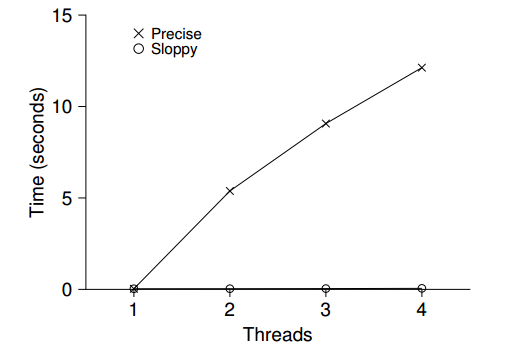
\includegraphics[width=.6\linewidth]{resources/concurrent_counter_performance.png}
% \end{figure}
\end{frame}

\begin{frame}{Locked Data Structures}
\framesubtitle{Sloppy Counter}
\begin{itemize}
 
\item local counter + local lock
\item global counter + global lock
\end{itemize}
\begin{table}
\scriptsize
\begin{tabular}{r|c c c c|l}
Time&$L_1$&$L_2$&$L_3$&$L_4$&$G$\\
\hline
0&0&0&0&0&0\\
1&0&0&1&1&0\\
2&1&0&2&1&0\\
3&2&0&3&1&0\\
4&3&0&3&2&0\\
5&4&1&3&3&0\\
6&5$\rightarrow$0&1&3&4&5 (from $L_1$)\\
7&0&2&4&5$\rightarrow$0&10 (from $L_4$)\\
\end{tabular}
\end{table}
\end{frame}

\begin{frame}[fragile]{Locked Data Structures}
\framesubtitle{Sloppy Counter (contd.)}
\begin{minipage}{.49\linewidth}
\begin{lstlisting}[language=C]
typedef struct __counter_t {
 int global;
 pthread_mutex_t glock;
 int local[NUMCPUS];
 pthread_mutex_t llock[NUMCPUS];
 int threshold;
} counter_t;

void init(counter_t *c, int threshold) {
 c->threshold = threshold;
 c->global = 0;
 Pthread_mutex_init(&c->glock, NULL);
 for (int i = 0; i < NUMCPUS; i ++) {
 c->local[i] = 0;
 pthread_mutex_init(&c->llock[i], NULL);
 }
}
\end{lstlisting}
\end{minipage}
\hspace{13pt}
\begin{minipage}{.49\linewidth}
\begin{lstlisting}[language=C]
void update(counter_t *c, int threadID, int amt) {
 int cpu = threadID % NUMCPUS;
 pthread_mutex_lock(&c->llock[cpu]);
 c->local[cpu] += amt;
 if (c->local[cpu] >= c->threshold) {
 pthread_mutex_lock(&c->glock);
 c->global += c->local[cpu];
 pthread_mutex_unlock(&c->glock);
 c->local[cpu] = 0;
 }
 pthread_mutex_unlock(&c->llock[cpu]);
}

int get(counter_t *c) {
 pthread_mutex_lock(&c->glock);
 int rc = c->global;
 pthread_mutex_unlock(&c->glock);
 return rc;
}
\end{lstlisting}
\end{minipage}
\end{frame}

\begin{frame}[fragile]{Locked Data Structures}
\framesubtitle{A Simple Concurrent Linked List}
\begin{lstlisting}[language=C]
typedef struct __node_t {
	int key;
 	struct __node_t *next;
} node_t;

typedef struct __list_t {
	node_t *head;
	pthread_mutex_t lock;
} list_t;

void List_Init(list_t *L) {
	L->head = NULL;
	pthread_mutex_init(&L->lock, NULL);
}
\end{lstlisting}
\end{frame}

\begin{frame}[fragile]{Locked Data Structures}
\framesubtitle{A Simple Concurrent Linked List (contd.)}
\begin{lstlisting}[language=C]
int List_Insert(list_t *L, int key) {
	pthread_mutex_lock(&L->lock);
	node_t *new = malloc(sizeof(node_t));
	if (new == NULL) {
		pthread_mutex_unlock(&L->lock);
		return -1; 
	}
	new->key = key;
	new->next = L->head;
	L->head = new;
	pthread_mutex_unlock(&L->lock);
	return 0; 
}
int List_Lookup(list_t *L, int key) {
	pthread_mutex_lock(&L->lock);
	node_t *curr = L->head;
	while (curr) {
		if (curr->key == key) {
			pthread_mutex_unlock(&L->lock);
			return 0;
		}
		curr = curr->next;
	}
	pthread_mutex_unlock(&L->lock);
	return -1;
}
\end{lstlisting}
\end{frame}

\begin{frame}{Locked Data Structures}
\framesubtitle{Scaling Linked Lists}
\begin{itemize}
 
\item \textcolor{blue}{Hand-over-hand locking} (a.k.a. lock coupling)
\item Instead of having a single lock for the entire list, you instead add a lock per node of the list.
\item When traversing the list, the code first grabs the next node's lock and then releases the current node's lock
\item High degree of concurrency in list operations.
In practice, it is hard to make such a structure faster than the simple single lock approach. (Surprise? Guess why.)
\item A hybrid would be worth investigating.
\end{itemize}
\end{frame}

\begin{frame}[fragile]{Locked Data Structures}
\framesubtitle{Concurrent Queue}
\begin{itemize}
 
\item Instead of adding a big lock, any approach more concurrently?
\end{itemize}
\begin{lstlisting}[language=C]
typedef struct __node_t {
	int value;
 	struct __node_t *next;
} node_t;

typedef struct __queue_t {
	node_t *head;
	node_t *tail;
	pthread_mutex_t headLock;
	pthread_mutex_t tailLock;
} queue_t;

void Queue_Init(queue_t *q) {
	node_t *tmp = malloc(sizeof(node_t));
	tmp->next = NULL
	q->head = q->tail = tmp;
	pthread_mutex_init(&q->headLock, NULL);
	pthread_mutex_init(&q->tailLock, NULL);
}
\end{lstlisting}
\end{frame}

\begin{frame}[fragile]{Locked Data Structures}
\framesubtitle{Concurrent Queue (contd.)}
\begin{lstlisting}[language=C]
void Queue_Enqueue(queue_t *q, int value) {
	node_t *tmp = malloc(sizeof(node_t));
	assert(tmp != NULL);
	tmp->value = value;
	tmp->next = NULL;
	pthread_mutex_lock(&q->tailLock);
	q->tail->next = tmp;
	q->tail = tmp;
	pthread_mutex_unlock(&q->tailLock);
}

int Queue_Dequeue(queue_t *q, int *value) {
	pthread_mutex_lock(&q->headLock);
	node_t *tmp = q->head;
	node_t *newHead = tmp->next;
	if (newHead == NULL) {
		pthread_mutex_unlock(&q->headLock);
		return -1;
	}
	*value = newHead->value;
	q->head = newHead;
	pthread_mutex_unlock(&q->headLock);
	free(tmp);
	return 0;
}
\end{lstlisting}
\end{frame}

\begin{frame}[fragile]{Locked Data Structures}
\framesubtitle{Concurrent Hash Table}
\begin{itemize}
 
\item Instead of adding a big lock, any approach more concurrently?
\end{itemize}
\begin{lstlisting}[language=C]
#define BUCKETS (101)

typedef struct __hash_t {
	list_t lists[BUCKETS];
} hash_t;

void Hash_Init(hash_t *h) {
	for (int i = 0; i < BUCKETS; i ++)
		List_Init(&h->lists[i]);
}

int Hash_Insert(hash_t *h, int key) {
	int bucket = key % BUCKETS;
	return List_Insert(&h->lists[buckets], key);
}

int Hash_Lookup(hash_t *h, int key) {
	int bucket = key % BUCKETS;
	return List_Lookup(&H->lists[bucket], key);
}
\end{lstlisting}
\end{frame}




\end{document}
